\documentclass[handout, 10pt]{beamer}

%\usepackage[backend=bibtex,firstinits=true,style=verbose-inote,citestyle=authortitle]{biblatex}
\usepackage{bm}
\usepackage{graphicx}
\usepackage{subcaption}
\usepackage{amsmath}
\usepackage{amsfonts}
\usepackage{makecell}
\usepackage{filecontents}
\usepackage{biblatex}
\usepackage{xcolor}
% \newcommand{\expect}[2][]{
\ifthenelse{\equal{#1}{}}{
\mathbb{E}\left[#2\right]
}{
\underset{#1}{\mathbb{E}}\left[#2\right]
}}

\newcommand{\cov}[2][]{
\ifthenelse{\equal{#1}{}}{
\text{Cov}\left[#2\right]
}{
\underset{#1}{\text{Cov}}\left[#2\right]
}}


\newcommand{\var}[2][]{
\ifthenelse{\equal{#1}{}}{
\text{Var}[#2]
}{
\underset{#1}{\text{Var}}[#2]
}}

\newcommand{\loss}[2][]{
\ifthenelse{\equal{#1}{}}{
\mathcal{L}(#2)
}{
\mathcal{L}_{#1}(#2)
}}

\newcommand{\kl}[2]{
\text{D}_\text{KL}[#1 \parallel #2]
}

\newcommand{\R}{\mathbb{R}}
%\newcommand{\Prob}{\mathbb{P}}

\newcommand{\1}[1]{\mathds{1}\{#1\}}


%\usecolortheme{dolphin}
\setbeamertemplate{navigation symbols}{}
\setbeamertemplate{section in toc}{\inserttocsectionnumber.~\inserttocsection}

\begin{filecontents*}{references.bib}
@misc{ReZero,
    title={ReZero is All You Need: Fast Convergence at Large Depth},
    author={Thomas Bachlechner and Bodhisattwa Prasad Majumder and Huanru Henry Mao and Garrison W. Cottrell and Julian McAuley},
    year={2020},
    eprint={2003.04887},
    archivePrefix={arXiv},
    primaryClass={cs.LG}
}
\end{filecontents*}

\addbibresource{references.bib}


\title{ReZero is All You Need: Fast Convergence at Large Depth\footnote{\citepaper{ReZero}}}
%\subtitle{}
%\author{Ivan Skorokhodov}
%\date{}
%\logo{
\includegraphics[height=1cm]{images/ipavlov-logo.png}}

\newcommand{\citepaper}[1]{\citetitle{#1} by \citeauthor{#1}, \citeyear{#1}}

%\graphicspath{{./images}}

%\usetheme{lucid}
\begin{document}

\begin{frame}
    \titlepage
\end{frame}

\begin{frame}{Overview}
\begin{itemize}
    \item\pause Initialization and stability is still an issue for many problems
    \item\pause Authors propose a simple trick, similar to residual connections:
\begin{equation}
\boldsymbol{x}_{i+1}=\boldsymbol{x}_{i}+\alpha_{i} F\left(\boldsymbol{x}_{i}\right)
\end{equation}
    where $\alpha_i$ is learnable and initialized at 0.
    \item\pause It has the following benefits:
    \begin{itemize}
        \item\pause Simplicity and wide applicability
        \item\pause Faster convergence
        \item\pause It allows training of deeper models
    \end{itemize}
    \item\pause Authors test their approach on
    \begin{itemize}
        \item\pause Language modelling with Transformer
        \item\pause Classification on CIFAR-10
    \end{itemize}
    \item\pause They show good performance in terms of fast convergence and stability
\end{itemize}
\end{frame}


%\begin{frame}{Dynamical Isometry}
%    \begin{itemize}
%        \item\pause Dynamical Isometry is a property that all singular values of the input-output Jacobian are close to 1
%        \item\pause This property allows to train models much faster and make them much deeper
%    \end{itemize}
%\end{frame}


\begin{frame}{Residual with zero init (ReZero)}
\begin{itemize}
    \item\pause Dynamical Isometry is a property that all singular values of the input-output Jacobian are close to 1
    \item\pause It allows to train models much faster and make them much deeper
    \item\pause Authors propose an easy trick that makes a model satisfy it (at init):
    \begin{equation}
\boldsymbol{x}_{i+1}=\boldsymbol{x}_{i}+\alpha_{i} F\left(\boldsymbol{x}_{i}\right)
\end{equation}
    where $\alpha_i$ is learnable and initialized at 0.
    \begin{figure}
        \centering
        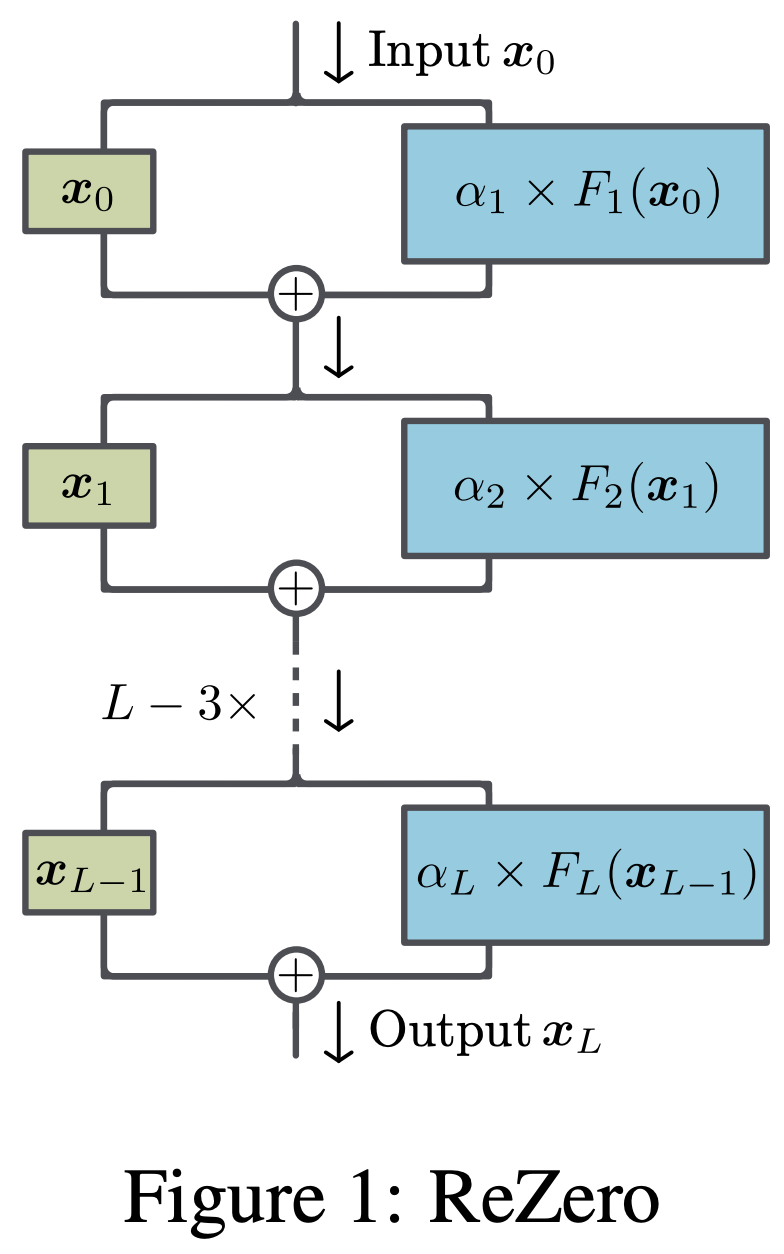
\includegraphics[width=0.2\textwidth]{images/rezero-block}
    \end{figure}
    \item\pause Experiments show that this property remains approximately preserved later on in training as well
\end{itemize}    
\end{frame}


\begin{frame}{Fully-Connected models on CIFAR-10}
\begin{figure}
\centering
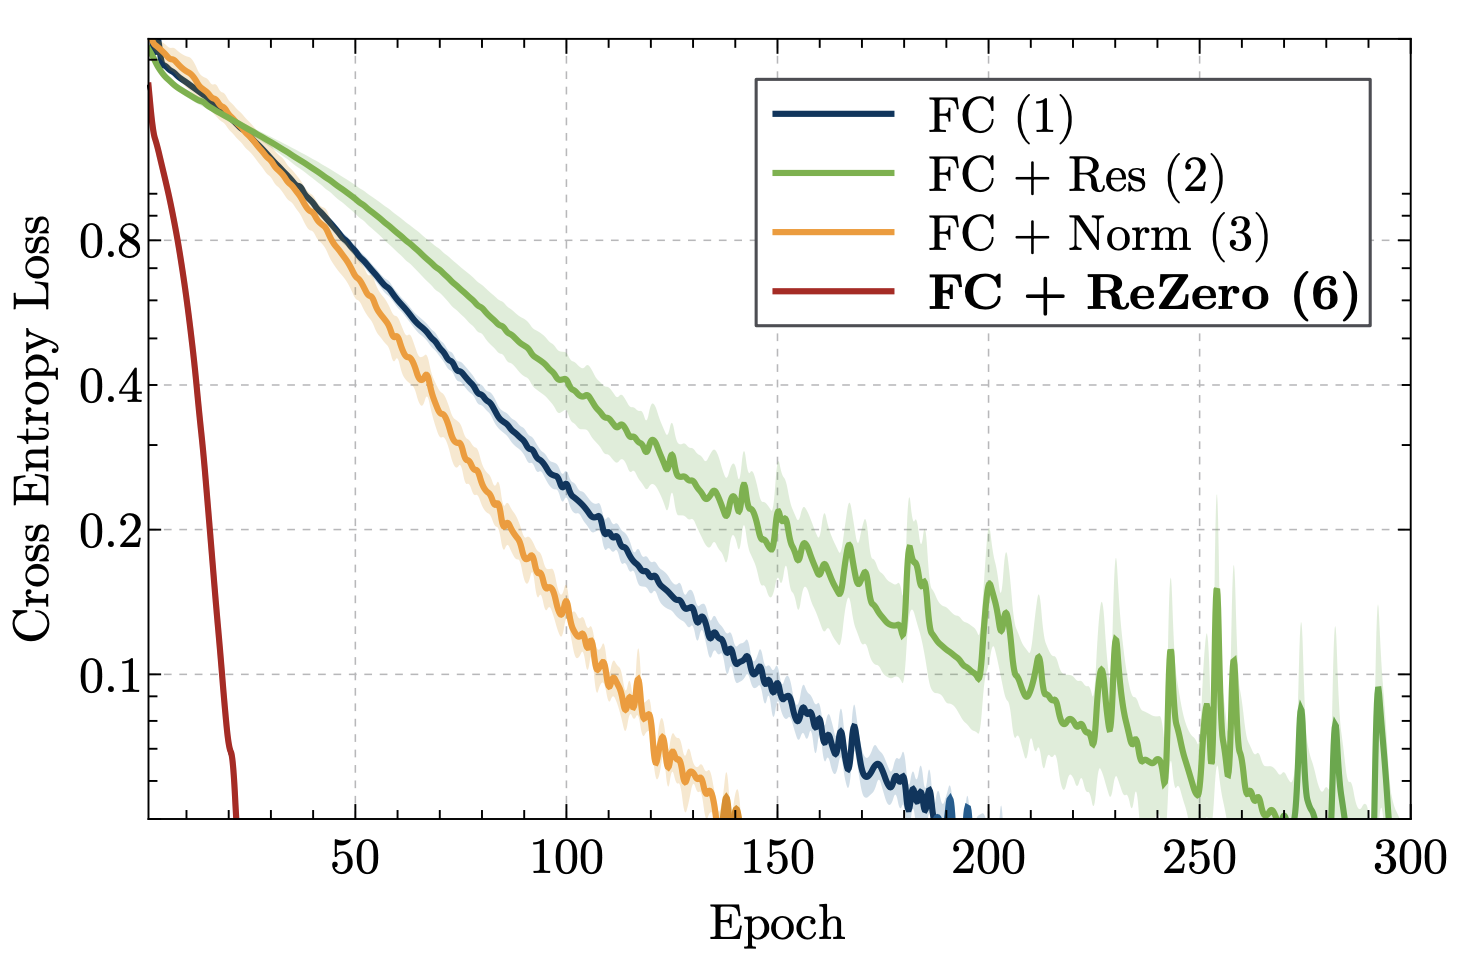
\includegraphics[width=0.7\textwidth]{images/fc-models-cifar10.png}
\caption{Convergence speed for different normalization strategies}
\end{figure}
\end{frame}


\begin{frame}{Convolutional models on CIFAR-10}
\begin{figure}
\centering
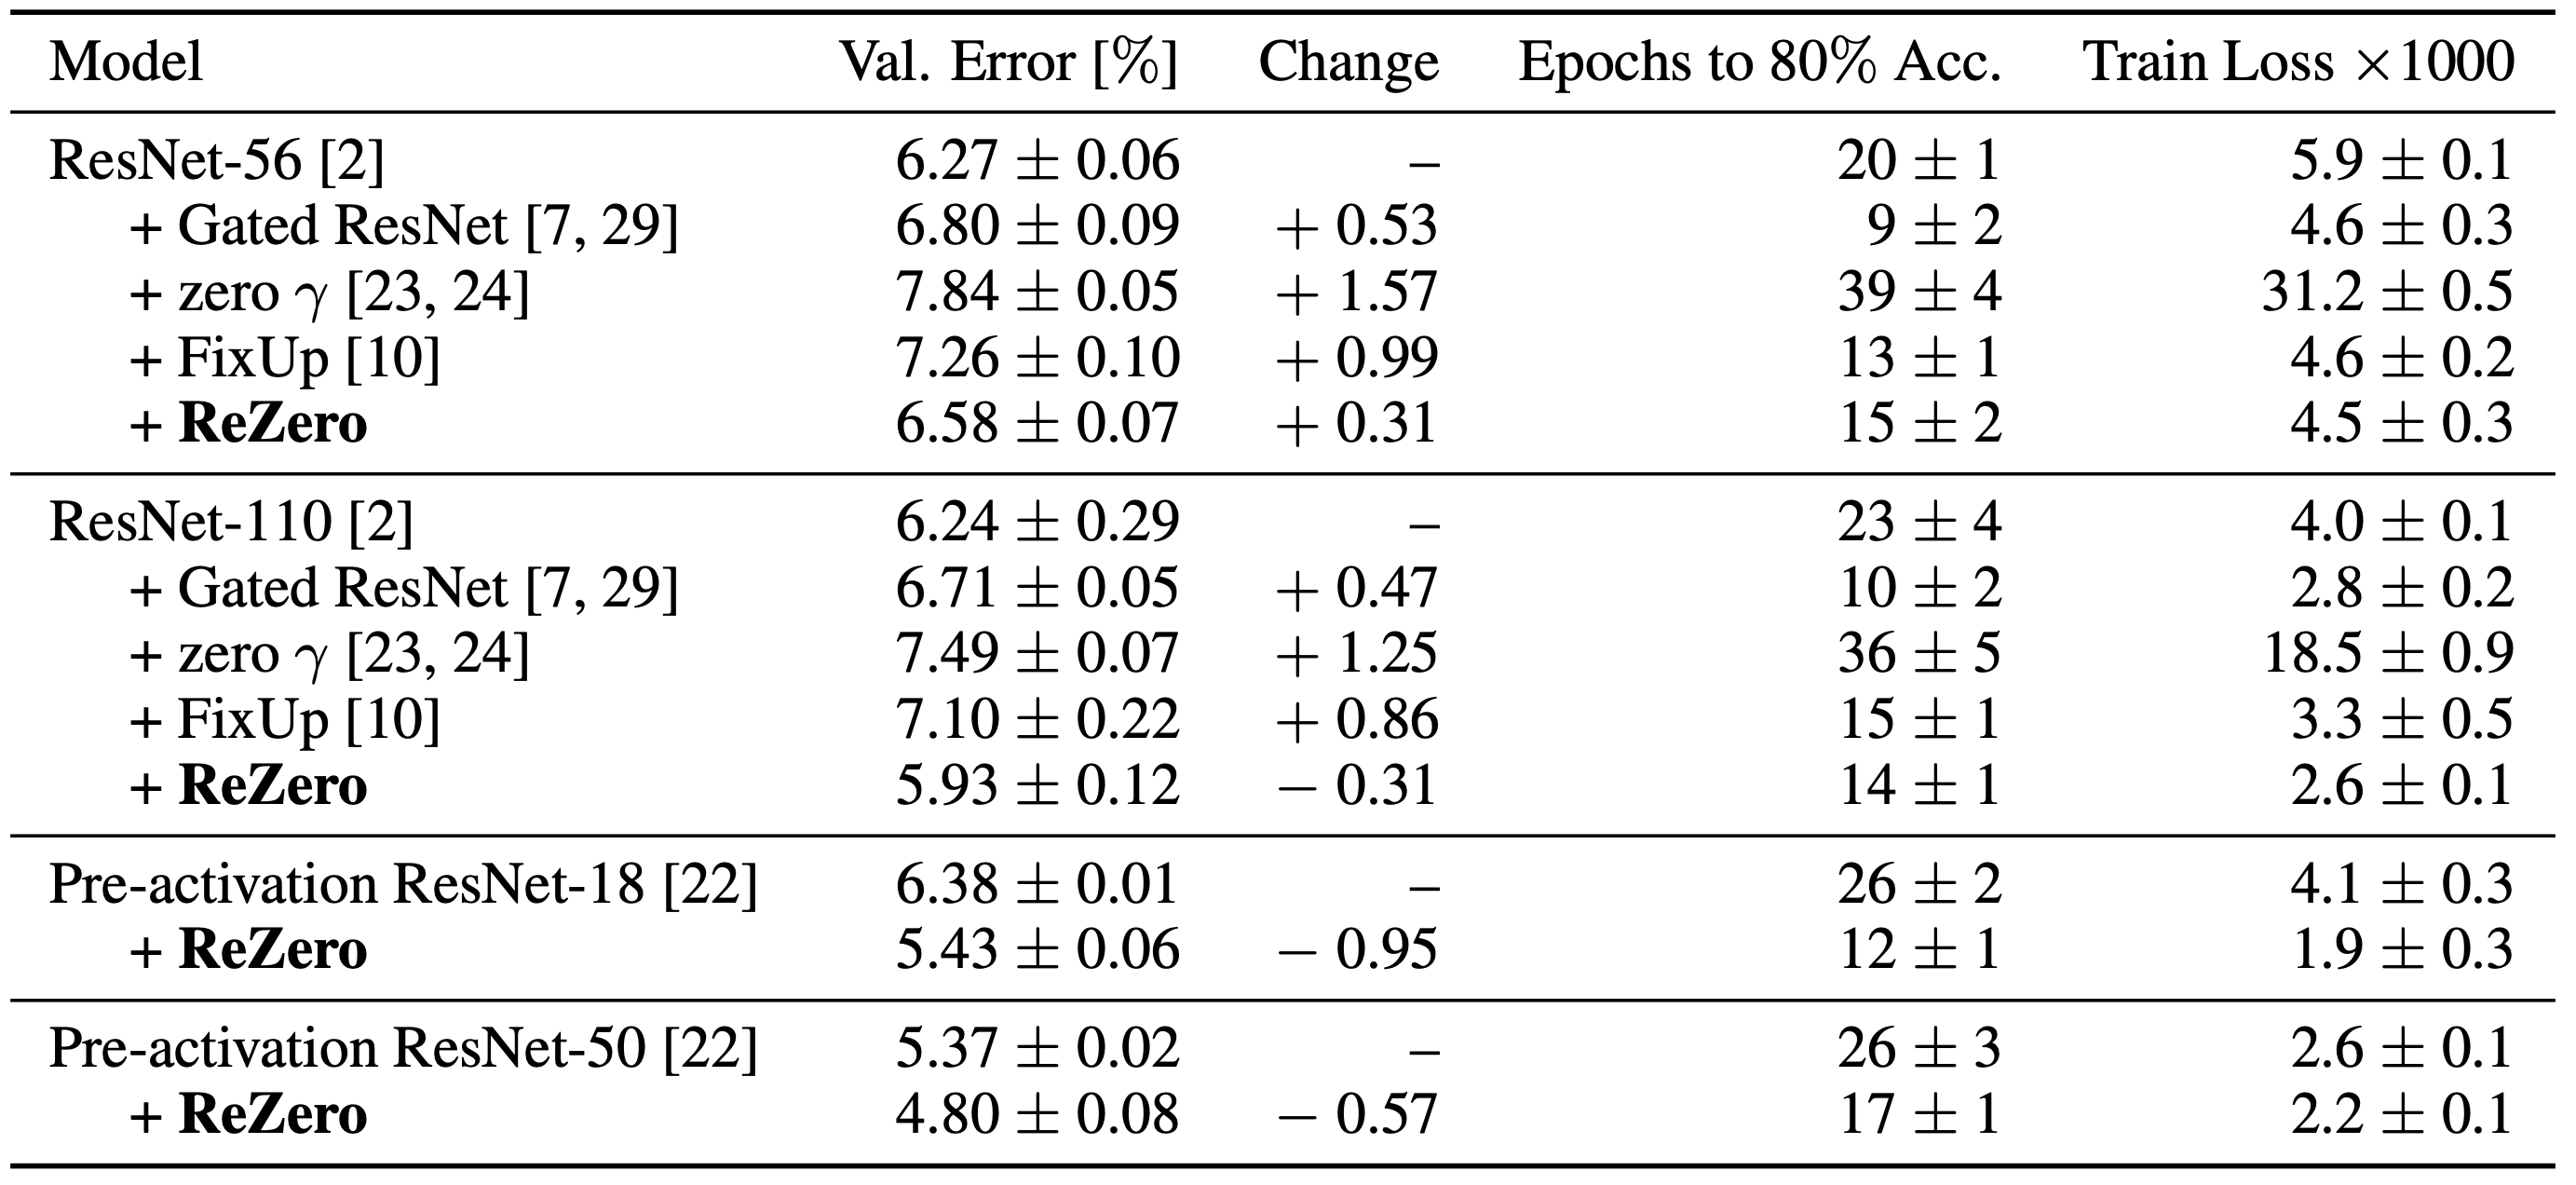
\includegraphics[width=\textwidth]{images/conv-models-cifar10}
\end{figure}
\end{frame}


\begin{frame}{ReZero Transformer}
Vanilla Transformer uses Post-Norm normalization:
\begin{equation}
\boldsymbol{x}_{i+1}=\text { LayerNorm }\left(\boldsymbol{x}_{i}+\operatorname{sublayer}\left(\boldsymbol{x}_{i}\right)\right)
\end{equation}
Authors replaced this with:
\begin{equation}
\boldsymbol{x}_{i+1}=\boldsymbol{x}_{i}+\alpha_{i} \operatorname{sublayer}\left(\boldsymbol{x}_{i}\right)
\end{equation}

\begin{figure}
\centering
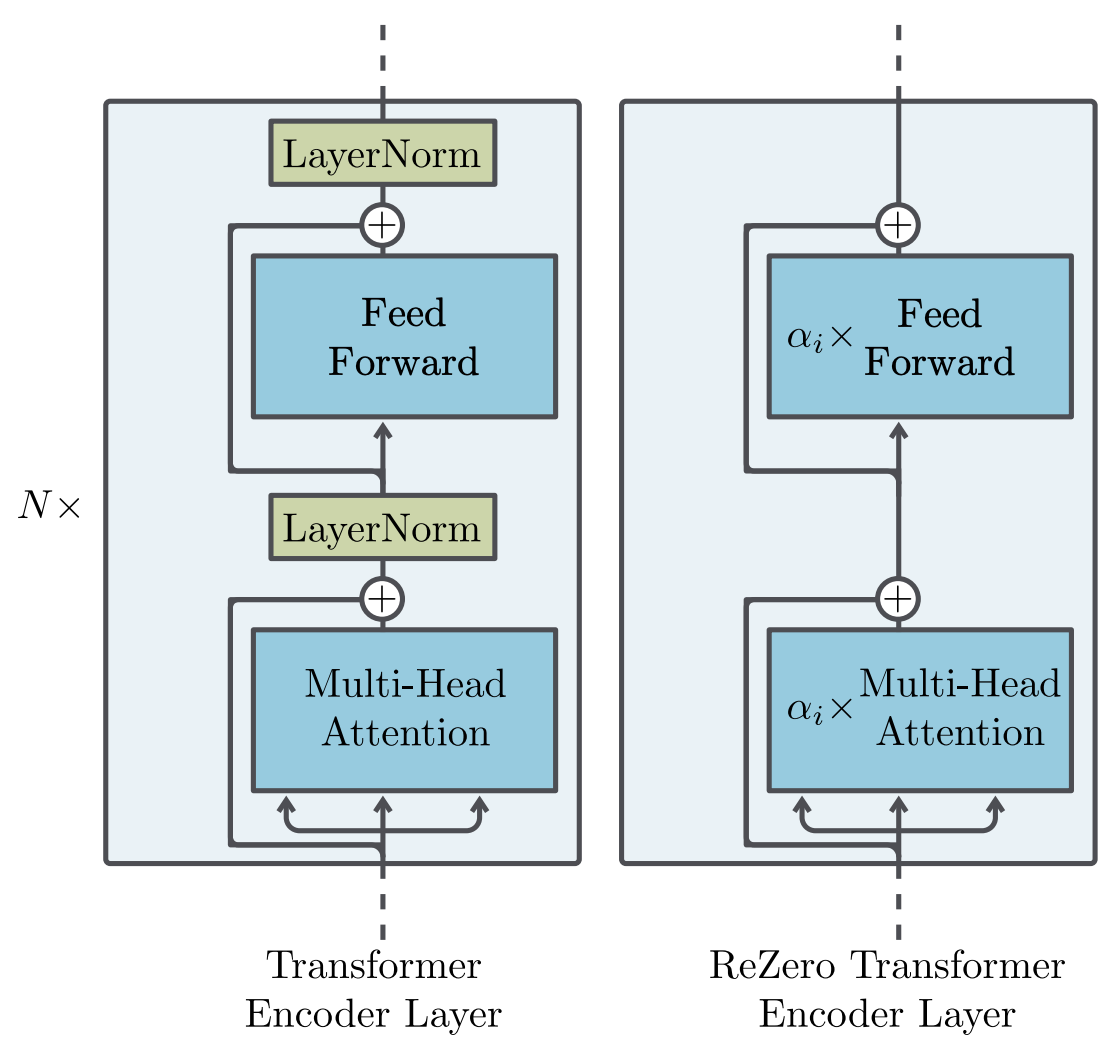
\includegraphics[width=0.5\textwidth]{images/rezero-transformer.png}
\end{figure}
\end{frame}

\begin{frame}{Language Modeling results}
\begin{figure}
\centering
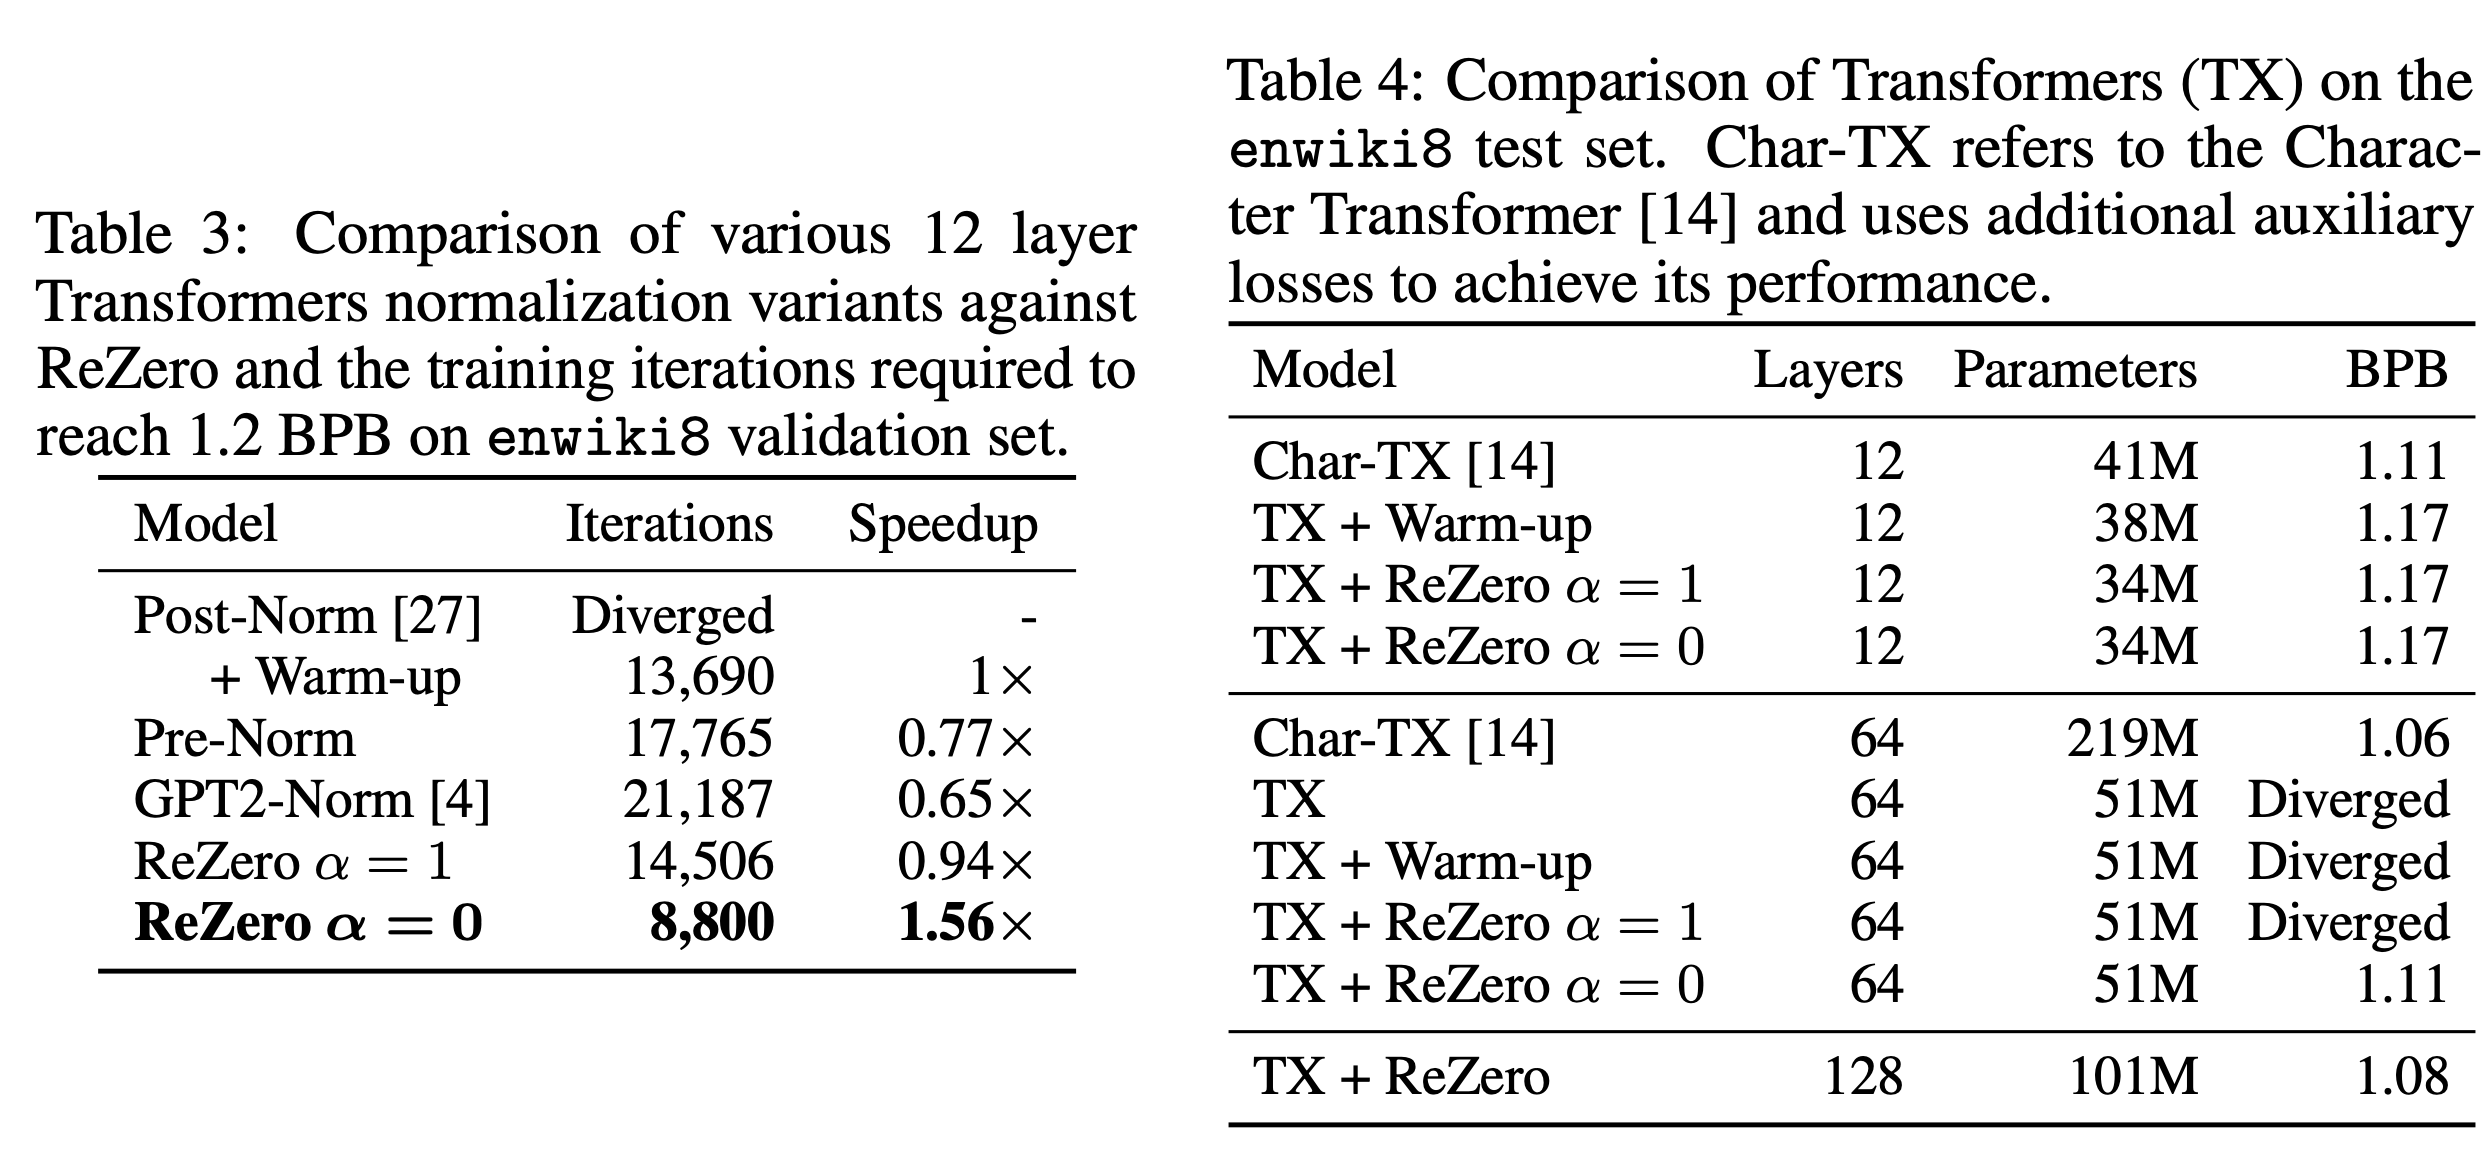
\includegraphics[width=\textwidth]{images/lm-results}
\end{figure}
\end{frame}


\begin{frame}{Model preserves dynamic isometry by itself}
\begin{figure}
\centering
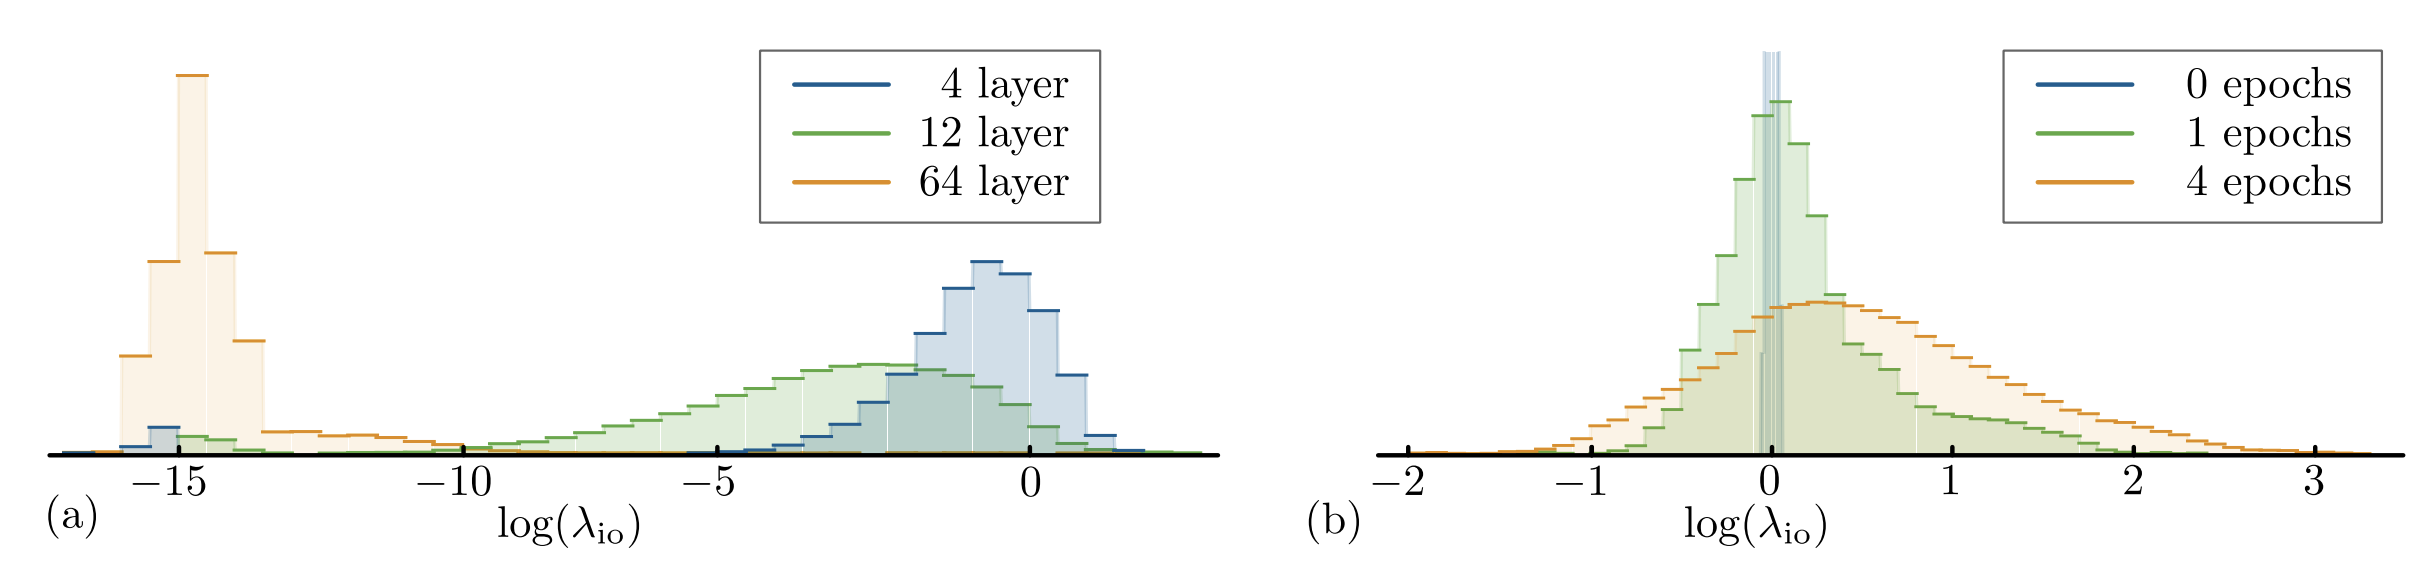
\includegraphics[width=\textwidth]{images/log-singular-values-hist}
\caption{Histograms of $\log(\sigma)$ of singular values. Left: traditional Transformer. Right: 64-layer ReZero Transformer}
\end{figure}
\end{frame}


\begin{frame}{Residual weights evolution}
\begin{figure}
\centering
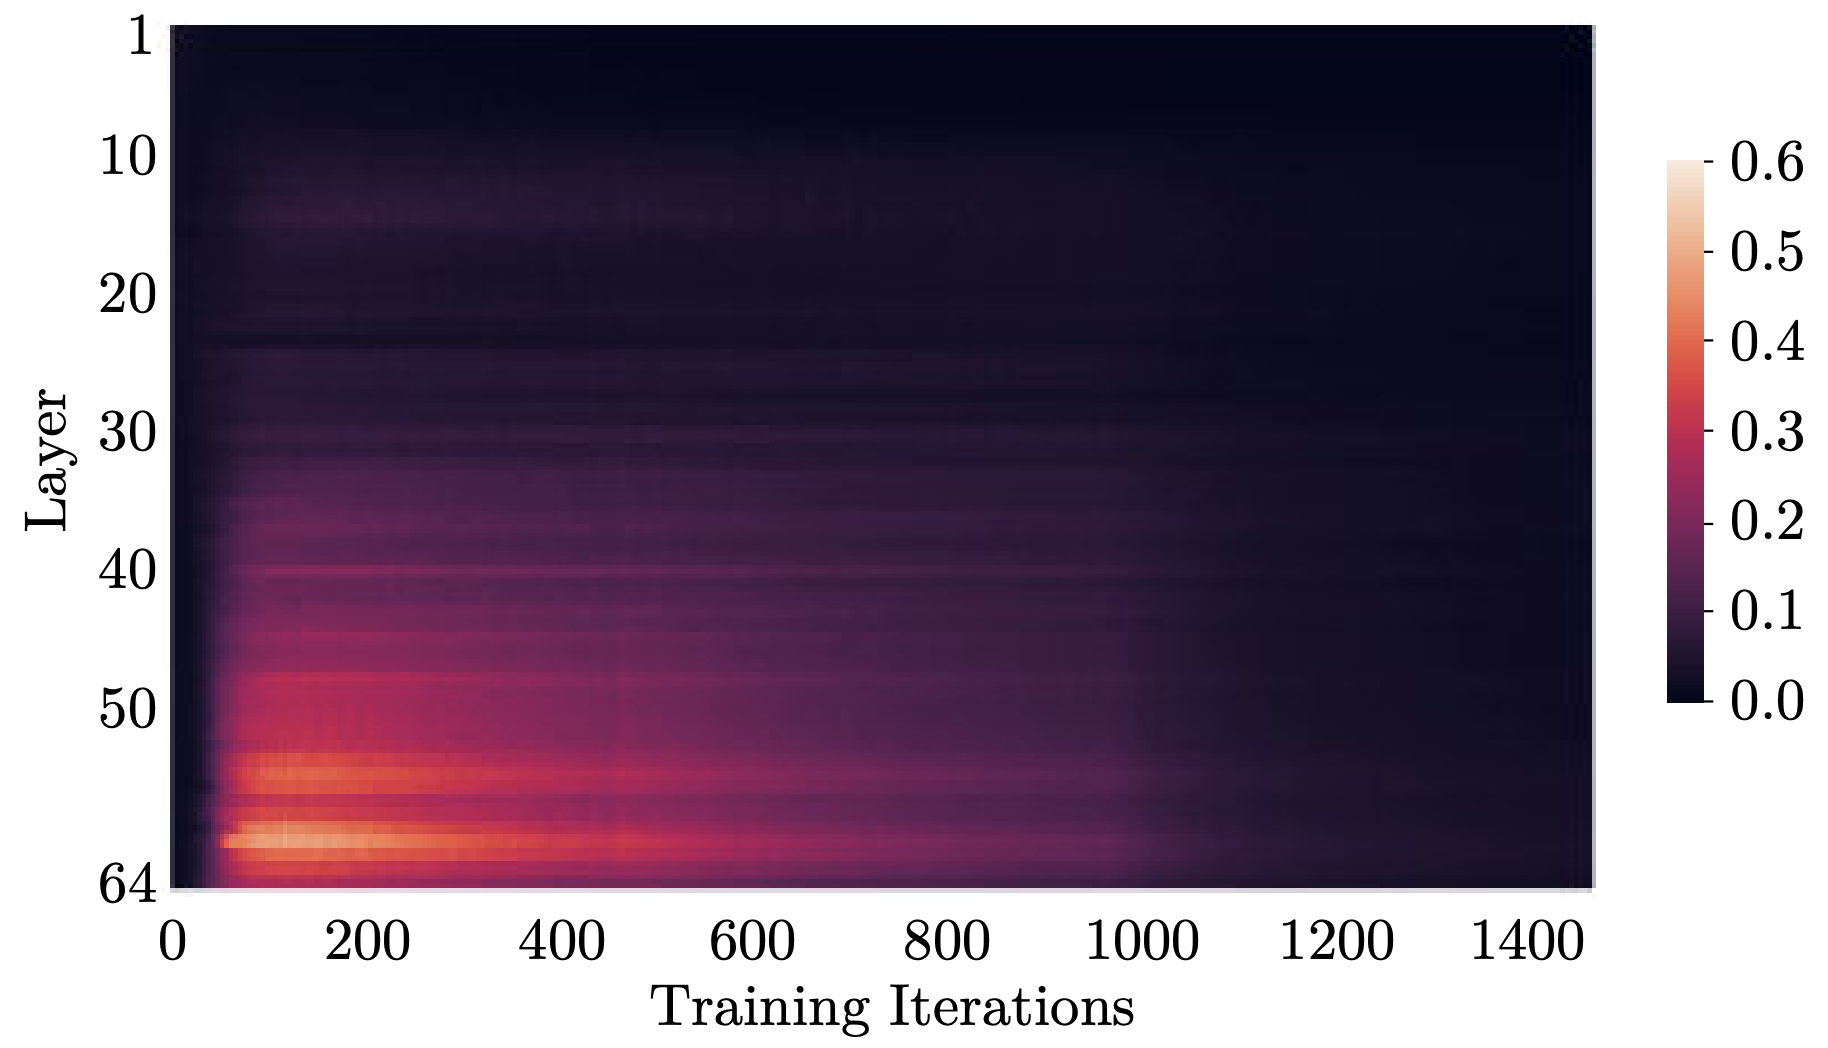
\includegraphics[width=0.8\textwidth]{images/rezero-weights-evolution}
\caption{Evolution of $\alpha_i$ for 64-layer Transformer}
\end{figure}

\begin{itemize}
    \item\pause Model first increases $\alpha_i$ for later layers, then decreases them all.
    \item\pause Authors say that there is a similar pattern for $\alpha = 1$ (for a 12-layer transformer): model first tries to reduce $\alpha$. But instead of increasing later $\alpha_i$, model pushes initial $\alpha_i$ to small values at first $\approx 50$ iterations.
    \item\pause Finally, model selects $\alpha_i \approx 1/L$.
\end{itemize}
\end{frame}


%\begin{frame}{Conclusion}
%\begin{itemize}
%    \item\pause 
%%    \item\pause Why does it work to initialize $\alpha_i = 0$? 
%\end{itemize}
%\end{frame}

\end{document}
